\documentclass[addpoints]{exam}
\usepackage{amsmath,amsthm,amssymb,url}
\usepackage{cancel}
\usepackage{algorithm}
\usepackage{algorithmic}
\usepackage{graphicx}
\usepackage{float}
\usepackage{upgreek}
\usepackage{bm}
\usepackage{units}
\usepackage[pdftex]{hyperref}
\usepackage{tikz}

\def\checkmark{\hspace{.5em}\tikz\fill[scale=0.4](0,.35) -- (.25,0) -- (1,.7) -- (.25,.15) -- cycle;} 
\DeclareMathOperator*{\pprime}{\prime \prime}
\renewcommand{\algorithmicrequire}{\textbf{Input:}}
\renewcommand{\algorithmicensure}{\textbf{Output:}}
\newcommand{\BigO}[1]{\mathcal{O}\left( #1\right)}


\newtheorem{lemma}{Lemma}[section]
\newcommand{\var}{\text{Var}}
\title{ME EN 6720: Homework 1}
\date{Due Date: February 15, 2016}
\author{Christopher Mertin}
\begin{document}
\maketitle
%\begin{center}
%\fbox{\fbox{\parbox{5.5in}{\centering
%This assignment has \numquestions\ questions, for a total of \numpoints\
%points.
%Unless otherwise specified, complete and reasoned arguments will be
%expected for all answers. 
%}}}
%\end{center}

\qformat{Question \thequestion: \thequestiontitle\dotfill}
\pointname{}
\bonuspointname{}
\pointformat{[\bfseries\thepoints]}

\printanswers



\begin{questions}

\titledquestion{Problem 1.1 (A)}
List the assumptions required to obtain the following energy equation from the full conservation of energy equation (e.g., Anderson Equation 2.81)

\begin{align}
\frac{\partial E}{\partial t} + \bm{\nabla}\cdot [(E+P)\mathbf{V}] = 0\label{eq:simple}
\end{align}

where $E$ is the total energy and bold symbols indicate vectors.
\begin{solution}
The full {\em conservative form} of the energy equation can be represented as
\begin{align}
\frac{\partial}{\partial t}\left[\rho\left(e+\frac{V^{2}}{2}\right)\right]+\bm{\nabla}\cdot\left[\rho\left( e+\frac{V^{2}}{2}\right)\mathbf{V}\right] &= \rho\dot{q}+\frac{\partial}{\partial x}\left(k\frac{\partial T}{\partial x}\right)+\frac{\partial}{\partial y}\left( k\frac{\partial T}{\partial y}\right)+ \frac{\partial}{\partial z}\left( k\frac{\partial T}{\partial z}\right)\nonumber\\
&-\frac{\partial (up)}{\partial x}-\frac{\partial (vp)}{\partial y}-\frac{\partial (wp)}{\partial z}+\frac{\partial (u\uptau_{xx})}{\partial x}+\frac{\partial (u\uptau_{yx})}{\partial y}\nonumber\\
&+\frac{\partial (u\uptau_{zx})}{\partial z}+\frac{\partial (v\uptau_{xy})}{\partial x} +\frac{\partial (v\uptau_{yy})}{\partial y}+\frac{\partial (v\uptau_{zy})}{\partial z}\nonumber\\
&+\frac{\partial (w\uptau_{xz})}{\partial x}+\frac{\partial (w\uptau_{yz})}{\partial y}+\frac{\partial (w\uptau_{zz})}{\partial z}+\rho\bm{f}\cdot\mathbf{V} \label{eq:full}
\end{align}

Where the total energy is represented as $(e+V^{2}/2)$. To get Equation~(\ref{eq:full}) to Equation~(\ref{eq:simple}), the following assumptions have to be made:

\begin{itemize}
\item There are no external forces, {\em i.e.} $\bm{f}=\vec{0}$
\item The fluid is incompressible, {\em i.e.} $\frac{\partial \rho}{\partial t} = 0$
\item The normal stress is constant as the volume of the fluid element isn't changing, {\em i.e.} $\frac{\partial \uptau_{xx}}{\partial x}=0$
\item The fluid element experiences no (or constant) shear stress, {\em i.e.} $\frac{\partial \uptau_{ij}}{\partial x} = 0;\quad i\neq j$
\item Temperature of the system is a uniform scalar field, {\em i.e.} $\frac{\partial T}{\partial x}=0$
\item The flow into the system is constant, {\em i.e.} $\dot{q}=0$
\item Volume element is stationary, {\em i.e.} $\frac{\partial u}{\partial x} = 0$
\end{itemize}
\end{solution}
\newpage

\titledquestion{Problem 1.1 (B)}
Show that the 1D Euler Equations can be written in terms of primitive variables $\mathbf{R}=[\rho, u, P]^{T}$ as
\begin{align}
&\frac{\partial \mathbf{R}}{\partial t}+\mathbf{M}\frac{\partial \mathbf{R}}{\partial x} = 0\label{eq:1d_form}\\
\intertext{where}
\mathbf{M} &= \left[ \begin{array}{c c c}u & \rho & 0\\ 0 & u & \rho^{-1} \\ 0 & \gamma P & u\end{array} \right]\label{eq:m_def}\\
\intertext{with the assumption that for an ideal gas, pressure and energy are related by}
P &= \underbrace{(\gamma - 1)}_{\alpha}\left(E-\frac{\rho u^{2}}{2}\right)\label{eq:p_def}
\end{align}

[{\em Hint: Use the 1D form of the equation from part A}]

\begin{solution}
The 1D Euler equations are defined as:
\begin{align}
\frac{\partial \rho}{\partial t} + \frac{\partial (\rho u)}{\partial x} &= 0\label{eq:cons_mass}\\
\frac{\partial (\rho u)}{\partial t} + \frac{\partial (\rho uu + P)}{\partial x} &= 0\label{eq:cons_momentum}\\
\frac{\partial (\rho E)}{\partial t} + \frac{\partial (\rho u E + u P)}{\partial x} &= 0\label{eq:cons_energy}
\end{align}
where Equation~(\ref{eq:cons_mass}) defines {\em Conservation of Mass}, Equation~(\ref{eq:cons_momentum}) defines {\em Conservation of Momentum}, and Equation~(\ref{eq:cons_energy}) defines {\em Conservation of Energy}. We can get these equations by working out Equation~(\ref{eq:1d_form}):
\begin{align}
\left[\begin{array}{c}\unitfrac{\partial \rho}{\partial t}\\ \unitfrac{\partial u}{\partial t}\\ \unitfrac{\partial P}{\partial t}\end{array}\right]+\left[\begin{array}{c c c}u & \rho & 0\\ 0 & u & \rho^{-1}\\ 0 & \gamma P & u\end{array}\right] \left[\begin{array}{c}\unitfrac{\partial \rho}{\partial x}\\ \unitfrac{\partial u}{\partial x}\\ \unitfrac{\partial P}{\partial x}\end{array}\right] &= \vec{0}\\
%%%%%%%%%%%%%%%%%%%%%%%%%
\left[\begin{array}{c}\unitfrac{\partial \rho}{\partial t}\\ \unitfrac{\partial u}{\partial t}\\ \unitfrac{\partial P}{\partial t}\end{array}\right] + \left[\begin{array}{c}u\unitfrac{\partial \rho}{\partial x} + \rho\unitfrac{\partial u}{\partial x}\\ u\unitfrac{\partial u}{\partial x} + \rho^{-1}\unitfrac{\partial P}{\partial x}\\ \gamma P\unitfrac{\partial u}{\partial x} + u\unitfrac{\partial P}{\partial x}\end{array} \right] &= \vec{0}\\
%%%%%%%%%%%%%%%%%%%%%%%%%
\intertext{We can now exploit the fact that $\omega \unitfrac{\partial \xi}{\partial \lambda} = \unitfrac{\partial (\omega \xi)}{\partial \lambda} - \unitfrac{\partial \xi}{\partial \lambda}$, which gives}
%%%%%%%%%%%%%%%%%%%%%%%%%
\left[\begin{array}{c}\unitfrac{\partial \rho}{\partial t} + \unitfrac{\partial (\rho u)}{\partial x} - \unitfrac{\partial u}{\partial x} + \unitfrac{\partial (u\rho )}{\partial x} - \unitfrac{\partial \rho}{\partial x}\\ \unitfrac{\partial u}{\partial t} + \unitfrac{\partial (uu)}{\partial x} - \unitfrac{\partial u}{\partial x} + \unitfrac{\partial \left(P\rho^{-1}\right)}{\partial x} - \unitfrac{\partial \left(\rho^{-1}\right)}{\partial x}\\ \unitfrac{\partial P}{\partial t} + \unitfrac{\partial \left(u\gamma P\right)}{\partial x} - \unitfrac{\partial \left(\gamma P\right)}{\partial x} + \unitfrac{\partial \left(P u\right)}{\partial x} - \unitfrac{\partial u}{\partial x}   \end{array} \right] &= \vec{0}
%%%%%%%%%%%%%%%%%%%%%%%%%%
\intertext{from this point, it's easier to simplify each row by itself. This is possible as long as no major matrix calculations are done. Therefore, for the first row}
%%%%%%%%%%%%%%%%%%%%%%%%%%
\frac{\partial \rho}{\partial t} + \frac{\partial (\rho u)}{\partial x} + \underbrace{\frac{\partial (u\rho)}{\partial x} - \frac{\partial u}{\partial x} - \frac{\partial \rho}{\partial x}}_{u\unitfrac{\partial \rho}{\partial x} - \unitfrac{\partial \rho}{\partial x}} &= 0
\intertext{Where $\unitfrac{\partial \rho}{\partial x}=0$ due to conservation of flux, resulting in}
\frac{\partial \rho}{\partial t} + \frac{\partial (\rho u)}{\partial x} &= 0\checkmark\label{eq:cons_mass_done}
\intertext{For the second row, we have:}
\frac{\partial u}{\partial t} + \frac{\partial (uu)}{\partial x} + \frac{\partial (P/\rho)}{\partial x} - \frac{\partial u}{\partial x} - \cancel{\frac{\partial \left(\rho^{-1}\right)}{\partial x}} &= 0
\intertext{where the last term cancels out due to conservation of flux as in the previous case. We can also set $\frac{\partial u}{\partial x}=0$ because of the following. $u$ is defined as: }
u\equiv \lim_{x_{2}\rightarrow x_{1}}\frac{x_{2}-x_{1}}{t_{2}-t_{1}} & \approx \frac{\partial x}{\partial t}
\intertext{Since we have $\unitfrac{\partial u}{\partial x}$, that is}
\frac{\partial u}{\partial x} = \frac{\partial}{\cancel{\partial x}}\frac{\cancel{\partial x}}{\partial t} = \frac{\partial}{\partial t}(\text{const}) &= 0
\intertext{which comes about from the chain rule. This reduces our equation to}
\frac{\partial u}{\partial t} + \frac{\partial (uu)}{\partial x} + \frac{\partial (P/\rho)}{\partial x} &= 0
\intertext{where from here we can multiply through by $\rho$ since we're dealing with the conservative form, meaning $\rho$ is independent of $t$ and $x$. We can also combine like differentials, which results in}
\frac{\partial (u\rho)}{\partial t} + \frac{\partial (\rho uu + P)}{\partial x} &= 0 \checkmark\label{eq:cons_momentum_done}
\intertext{Finally, the last row which is defined as:}
\frac{\partial P}{\partial t} + \frac{\partial (u\gamma P)}{\partial x} - \frac{\partial (\gamma P)}{\partial x} + \frac{\partial (Pu)}{\partial x} - \cancel{\frac{\partial u}{\partial x}} &= 0\label{eq:form1}
\intertext{We can use the definition of $P$ in Equation~(\ref{eq:p_def}) to expand this equation, resulting in}
\frac{\partial P}{\partial t} &= \alpha\left[\frac{\partial E}{\partial t}-\frac{1}{2}\frac{\partial \left(\rho u^{2}\right)}{\partial t}\right]\\
\gamma\frac{\partial (uP)}{\partial x} &= \gamma\alpha\left[ u\frac{\partial P}{\partial x} + P\cancel{\frac{\partial \left(\rho u^{2}\right)}{\partial x}}\right]\\
\frac{\partial (Pu)}{\partial x} &= \alpha\left[ u\frac{\partial P}{\partial x} + P\cancel{\frac{\partial u}{\partial x}}\right]
\intertext{plugging these definitions into Equation~(\ref{eq:form1}) gives}
\left[ \frac{\partial E}{\partial t} - \cancel{\frac{1}{2}\frac{\partial \left(\rho u^{2}\right)}{\partial t}}\right] + \gamma\frac{\partial (uP)}{\partial x}-\gamma\left[\cancel{\frac{\partial E}{\partial x}}-\cancel{\frac{1}{2}\frac{\partial \left(\rho u^{2}\right)}{\partial x}}\right] &+ \underbrace{u\frac{\partial E}{\partial x}}_{\frac{\partial (uE)}{\partial x} - \cancel{\frac{\partial E}{\partial x}}}-\cancel{u\frac{1}{2}\frac{\partial \left( Pu^{2}\right)}{\partial x}} = 0\\
\intertext{where we can divide out the $\gamma$'s and multiply through by $\rho$ since it's independent of the differentials, combining like differentials, and giving us}
\frac{\partial (\rho E)}{\partial t} + \frac{\partial (\rho u E + u P)}{\partial x} &= 0\checkmark\label{eq:cons_energy_done}
\intertext{By combining Equations~(\ref{eq:cons_mass_done}), (\ref{eq:cons_momentum_done}), (\ref{eq:cons_energy_done}) back into matrix form, we get}
\left[\begin{array}{c}\unitfrac{\partial \rho}{\partial t} + \unitfrac{\partial (\rho u)}{\partial x}\\ \unitfrac{\partial (\rho u)}{\partial t} + \unitfrac{\partial (\rho uu + P)}{\partial x}\\ \unitfrac{\partial (\rho E)}{\partial t} + \unitfrac{\partial (\rho u E + uP)}{\partial x}\end{array}\right] &= \vec{0}\checkmark
\end{align}
\end{solution}

\titledquestion{Problem 1.2}
Given $f(x)=\sin(2\pi x)$ for $0\leq x \leq 1$ for 3 resolutions $\Delta x=\{0.1, 0.01, 0.001\}$ and do the following:

\begin{itemize}
\item Compute and plot finite difference approximations using forward and central differences for $f^{\prime}(x)$ and using central differences for $f^{\prime \prime}(x)$ (3 plots total)
\item Compute the error norm $\epsilon_{2}$ and the maximum relative error for each approximation
\item Verify the accuracy (order) of the 3 approximations
\end{itemize}

\begin{solution}
Given the function, we can find the analytical solutions to the derivatives, which are the following:
\begin{align}
f(x) &= \sin(2\pi x)\\
f^{\prime}(x) &= 2\pi \cos(2\pi x)\\
f^{\prime \prime}(x) &= -4\pi^{2}\sin(2\pi x)
\end{align}
we can use these equations as the {\em exact solution} for the plots, which is required in calculating the relative error. The derivatives were approximated with the following techniques
\begin{align}
\intertext{Central Difference $f^{\prime}(x)$:}
f^{\prime}(x) &\approx \frac{f(x+h) - f(x-h)}{2h}
\intertext{Forward Difference $f^{\prime}(x)$:}
f^{\prime}(x) &\approx \frac{f(x+h) - f(x)}{h}
\intertext{Central Difference $f^{\prime \prime}(x)$:}
f^{\prime \prime}(x) &\approx \frac{f(x+h)-2f(x)+f(x-h)}{h^{2}}
\end{align}

with these, we could calculate the relative error at each point, which is defined by

\begin{align}
\epsilon_{r} &= \left| \frac{a-\hat{a}}{a}\right|
\intertext{where $a$ is the {\em exact value} and $\hat{a}$ is the {\em numerical value}. The {\em Error Norm} could also be calculated with }
\epsilon_{p} &= \left[ \frac{1}{N} \sum_{i=1}^{N}\left| a_{i} - \hat{a}_{i}\right|^{p}\right]^{\frac{1}{p}}
\end{align}

where $p$ was chosen to be 2 to get the $\epsilon_{2}$-error norm. The following plots show the results from approximating $f^{\prime}(x)$ and $f^{\prime \prime}(x)$

\begin{figure}[H]
\centering
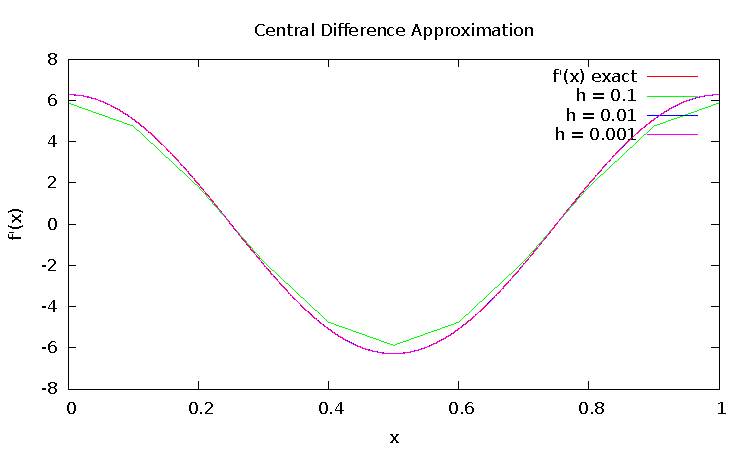
\includegraphics{CD.pdf}
\caption{Central Difference Approximation of $f^{\prime}(x)$}
\end{figure}

\begin{figure}[H]
\centering
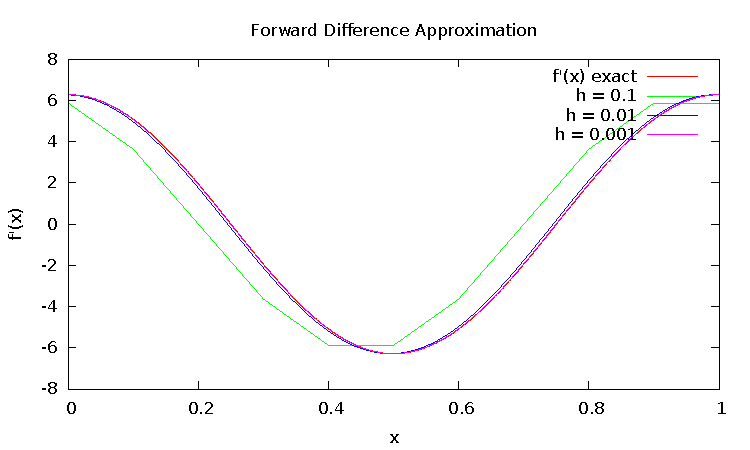
\includegraphics{FWD.pdf}
\caption{Forward Difference Approximation of $f^{\prime}(x)$}
\end{figure}

\begin{figure}[H]
\centering
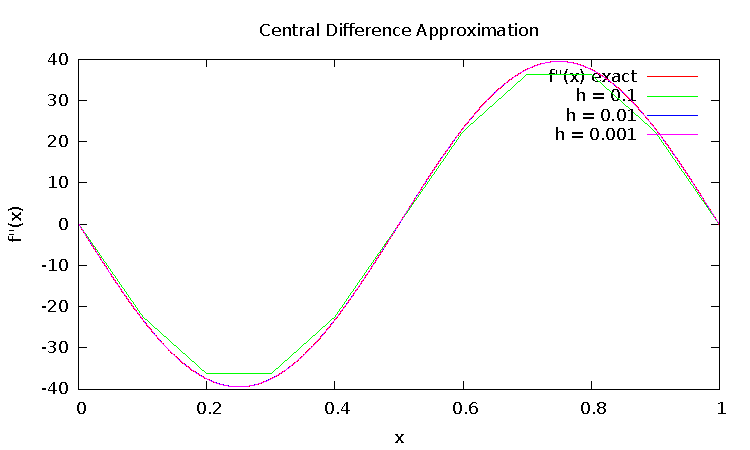
\includegraphics{CD2.pdf}
\caption{Central Difference Approximation of $f^{\prime \prime}(x)$}
\end{figure}

The following figures show the {\em relative error} for $f^{\prime}(x)$ and $f^{\prime \prime}(x)$ for each value of $x$.

\begin{figure}[H]
\centering
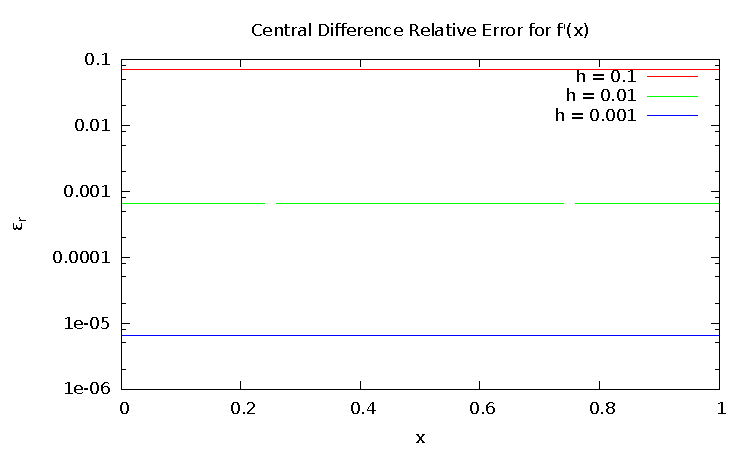
\includegraphics{CD_error.pdf}
\caption{Relative Error of the Central Difference Approximation of $f^{\prime}(x)$}
\end{figure}

\begin{figure}[H]
\centering
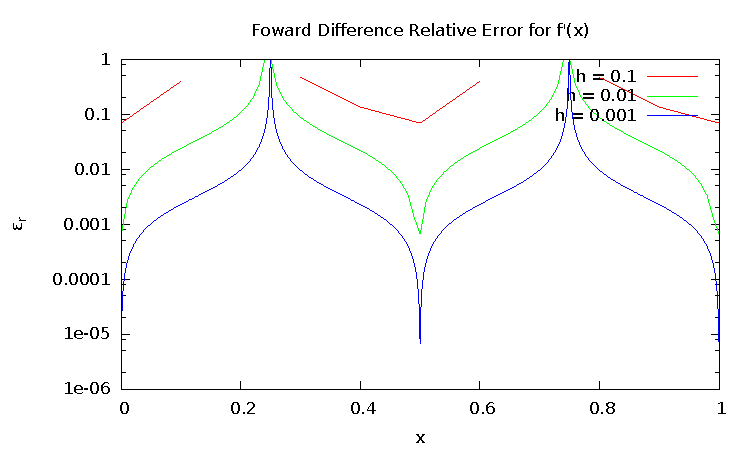
\includegraphics{FWD_error.pdf}
\caption{Relative Error of the Forward Difference Approximation of $f^{\prime}(x)$}
\end{figure}

\begin{figure}[H]
\centering
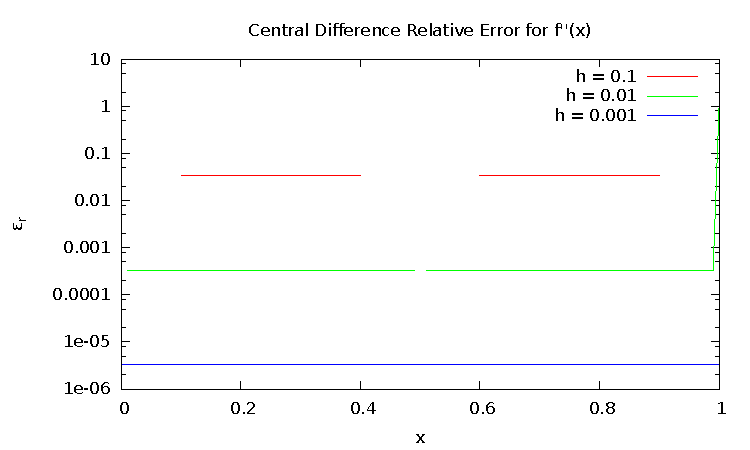
\includegraphics{CD2_error.pdf}
\caption{Relative Error of the Central Difference Approximation of $f^{\prime \prime}(x)$}
\end{figure}

Where the spaces in the figures come about due to the function. For example, in the center the {\em true value} was $\mathcal{O}\left(10^{-15}\right)$ while the {\em approximated value} was calculated as exactly $0$. On the edges for the central difference, it is easy enough to see that they wouldn't be included since the formula uses the values to the left and right of the point you're attempting to approximate.

\begin{table}[H]
\centering
\caption{Error Norm of Derivative Approximations}
\begin{tabular}{c c c c}
\hline\hline
$h$ & CD & FWD & CD$_{2}$\\
\hline
0.1\phantom{00} & 2.9936$\times 10^{-1}$ & 1.3220$\times 10^{0\phantom{-}}$ & 8.6420$\times 10^{-1}$\\
0.01\phantom{0} & 2.9372$\times 10^{-3}$ & 1.3887$\times 10^{-1}$ & 9.1370$\times 10^{-3}$\\
0.001 & 2.9548$\times 10^{-5}$ & 1.3951$\times 10^{-2}$ & 9.1792$\times 10^{-5}$\\
\hline\hline
\multicolumn{4}{l}{{\scriptsize CD: Central Difference Approximation of $f^{\prime}(x)$}}\\
\multicolumn{4}{l}{{\scriptsize FWD: Forward Difference Approximation of $f^{\prime}(x)$}}\\
\multicolumn{4}{l}{{\scriptsize CD$_{2}$: Central Difference Approximation of $f^{\prime \prime}(x)$}}\\
\end{tabular}
\end{table}

Finally, these results can be used to show that they obey the order of accuracy for each equation. For example, the forward difference approach is only accurate up until $\mathcal{O}(h)$ while both central difference approximations are accurate up to $\mathcal{O}\left(h^{2}\right)$. By looking at the plots of the relative error, it can be seen that they fall into this range of errors.

\end{solution}
\end{questions}

%\begin{thebibliography}{99}
%\end{thebibliography}

\end{document}

%%% Local Variables:
%%% mode: latex
%%% TeX-master: t
%%% End:
